%
% Príloha A
%
\chapter{Obsah CD}
Na priloženom CD sa nachádzajú nasledovné súbory a~adresáre:
\begin{itemize}
\item \textbf{doc} -- zdrojové súbory tohoto textu v~\LaTeX-ovom formáte 
spolu s~elektronickou verziou vo formáte PDF.
\item \textbf{TTT} -- zdrojové súbory plánovača testov spolu s~hlavičkami 
testov používaných v~praxi. Tento adresár takisto obsahuje súbory 
so známymi chybami \textit{KNOWN.BUGS} a~funkcie pre simuláciu testovania
pre potreby demonštrácie.
\item \textbf{working\_dir} -- pracovný adresár s~konfiguračnými súbormi
pre produkty MCO a~SMSCv5 a~štatistickými súbormi pre tieto dva produkty.
Do tohoto adresára sa v~prípade spustenia plánovača testov budú zapisovať
logovacie informácie.
\item \textbf{rpms} -- \textit{rpm} súbory pre nainštalovanie 
skriptovacieho jazyka Tcl/Tk vo verzii 8.4.19, pre ktorú je plánovač 
testov napísaný a~otestovaný.
\item \textbf{README.txt -} textový súbor obsahujúci príklady spustenia.
\end{itemize}



%
% Príloha B
%
\chapter{Ukážka jednoduchého plánu testov z~praxe}
\label{priloha:jednoduchy_plan_testov}
Na nasledujúcej strane je zobrazený plán testov z~produktu MCO,
ktorý pozostáva z~desiatich clusterov. Z~obrázku vyplýva, že pre potreby
týchto clusterov je potrebné spustiť celkovo 19 prerekvizít a~19 
odrekvizít. Pre otestovanie produktu týmito desiatimi clustermi, je 
potrebné vykonať ďalších 38 testov, ktoré slúžia na zmenu konfigurácie
systému, a~na obnovu týchto zmien. 

Uvedený plán obsahuje celkovo 48 testov, a~je relatívne jednoduchý.
V~regresných testoch sa aktuálne používa plán testov, ktorý v~prípade 
produktu MCO pozostáva z~viac ako 3100 testov.
Plán testov každodenne používaný v~regresnom testovaní produktu SMSCv5 
pozostáva z~približne 3000 testov.

V~produktoch MCO a~SMSCv5 sa každodenne spúšťajú regresné testy, ktoré
tvoria veľkú časť zo všetkých dostupných testov.
Spúšťanie regresných testov pre produkty MCO a~SMSCv5 je zabezpečované 
nasledujúcimi dvomi príkazmi.

\begin{lstlisting}[caption=Spúšťanie regresných testov v~produkte MCO
,label=priklad:prilohy_regresie_mco]
meszarosf@mco-v156#./Run_test.tcl -i mco.ini -B TEST.REVIEW_23 -f all -tw
\end{lstlisting}


\begin{lstlisting}[caption=Spúšťanie regresných testov v~produkte SMSCv5
,label=priklad:prilohy_regresie_smsc]
meszarosf@smsc-v156#./Run_test.tcl -i smsc.ini -f all 2nd -tw
\end{lstlisting}

\begin{figure}[h]
  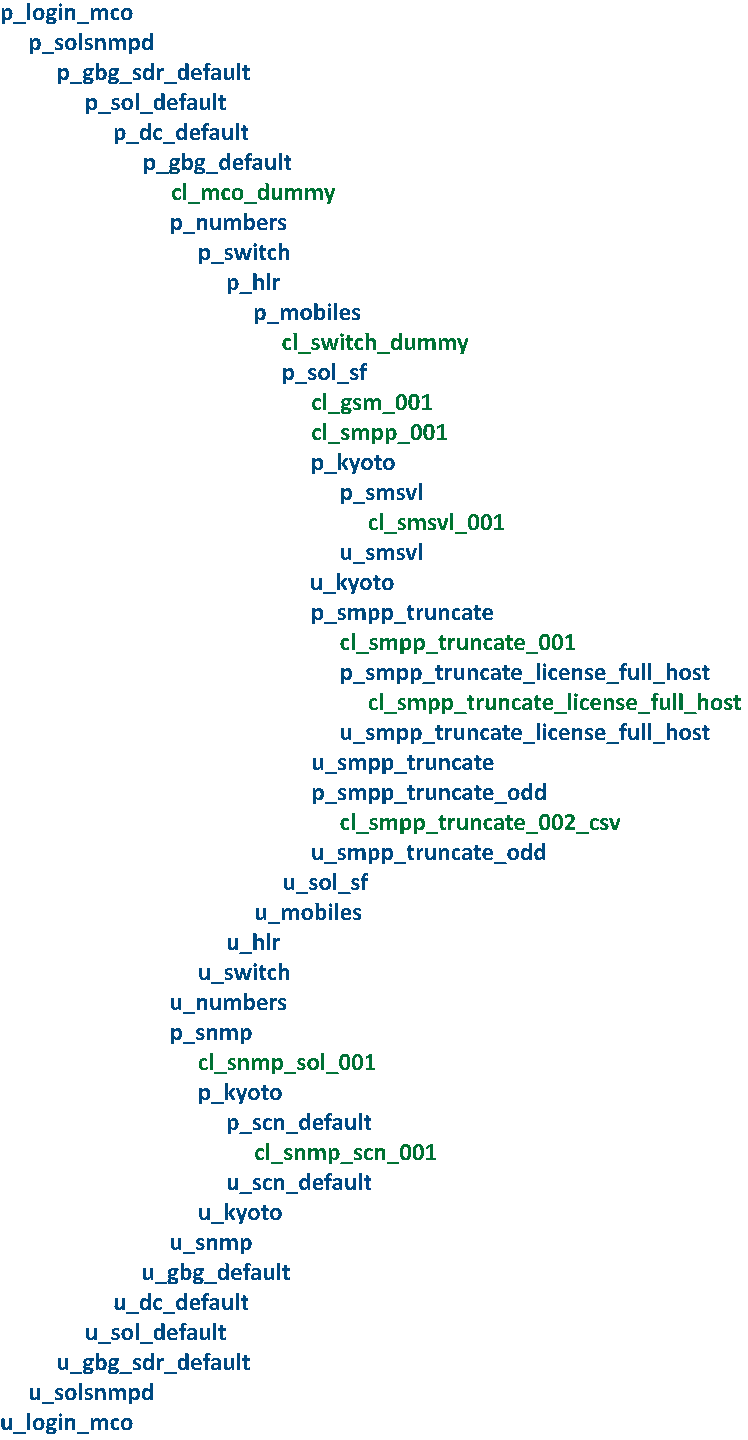
\includegraphics[scale=0.90]{ukazka_jednoducheho_planu}
  \caption{Ukážka jednoduchého plánu testov}
\end{figure}

%
% Príloha C
%
\chapter{Zmeny prevedené do zdrojových súborov a~odovzdané súbory}
\label{priloha:zmeny_do_zdrojakov}
Pri implementovaní rozšírenia plánovača testov som musel upraviť zdrojové
kódy dvoch hlavných súborov tohoto nástroja. 
Nakoľko boli tieto dva súbory vytvorené firmou Acision, v~tejto prílohe
sú uvedené zmeny do týchto dvoch súborov vykonané pri vytváraní tejto
práce. Približné zmeny týchto dvoch zdrojových súborov sú nasledovné:

\noindent Zmeny prevedené v~súbore \textbf{Run\_test.tcl}: \\
Riadky: 1433--1437, 1461--1464, 1467--1493 a~ďalej riadky 1499 až 1507.\\
Celkovo približne 50 riadkov kódu (bez komentárov).
\\
\\
\noindent Zmeny prevedené v~súbore \textbf{tstmng.tcl}: \\
Riadky: 125--133, 2257--2268, 2301--2322, 2551--2582, 2622--2624, 
3095--3097, 3199--3202, 3238--3242 a~riadky 3252 až 3260. \\
Ďalej riadky: 2360, 2365, 2369, 2374, 2379, 2384, 2410, 2415, 2424, 
2457, 2477, 2482, 2488, 2504, 2528, 2533, 2538, 2543, 2548 a~riadok 2642. \\
Celkovo približne 123 riadkov kódu (bez komentárov).
\\
\\
Pri odovzdávaní zdrojových súborov som navyše odovzdal len súbory,
potrebné pre beh plánovača testov. Jednotlivé testy pre produkty MCO
a~SMSCv5 boli odstránené a~nahradené jednoduchou funkciou 
\texttt{cl\_wait\_random\_ok} umiestnenou v~súbore \textit{CL-MY.tcl}. 

Hlavičky testov v~súboroch \textit{TEST.ALL} a~\textit{TEST.REVIEW\_23} 
boli ponechané priamo z~produktov MCO a~SMSCv5. V~týchto súboroch som 
však zmenil popis testov (informácia \textit{Description}) 
a~funkcionalitu (informácia \textit{Function}) popísané v~kapitole 
\ref{sekcia:princip_pouziteho_planovaca}.
Jednotlivé závislosti medzi testami ostali ponechané, a~je teda možné 
vytvoriť plány testov, ktoré sa používajú priamo v~praxi.
Súbory \textit{KNOWN.BUGS} ostali ponechané priamo z~týchto dvoch 
produktov bez zmeny. 

Medzi odovzdanými súbormi sa taktiež nachádzajú dva štatistické súbory 
slúžiace napríklad pre výpočet celkovej dĺžky trvania testovania. 
Medzi tieto súbory patria dva súbory \textit{TTT\_stat\_MCO.txt} (pre produkt MCO) 
a~súbor \textit{TTT\_stat\_SMSC.txt} (pre produkt SMSCv5).
Tieto súbory obsahujú presné informácie o~dĺžkach trvania jednotlivých 
testov v~týchto dvoch produktov. 
Pre využitie týchto súborov pre konkrétny produkt je potrebné jeden 
z~týchto súborov vložiť do logovacieho adresára \textit{Log/Stat} 
a~premenovať ho na súbor \textit{TTT\_stat.txt}.
V~prípade použitia týchto štatistických súborov plánovač testov počíta
odhadované časy dĺžky trvania testovania na základe údajov priamo z~praxe.



%
% Príloha D
%
\chapter{Ukážka progress baru}
\label{priloha:ukazka_progress_baru}
\begin{figure}[h]
  \begin{center}
%    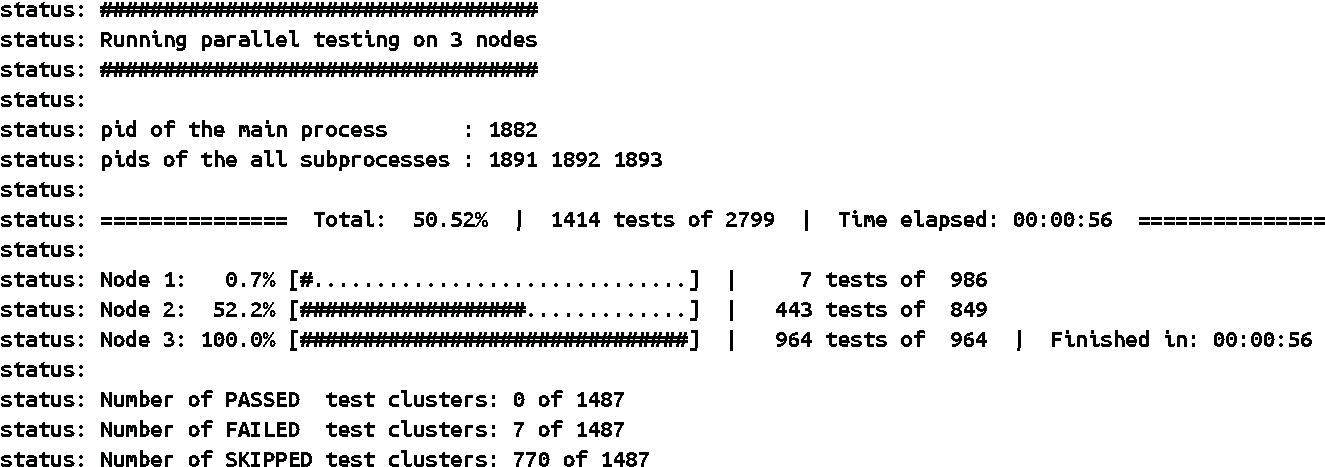
\includegraphics[scale=0.65,angle=90]{ukazka_progress_baru}
    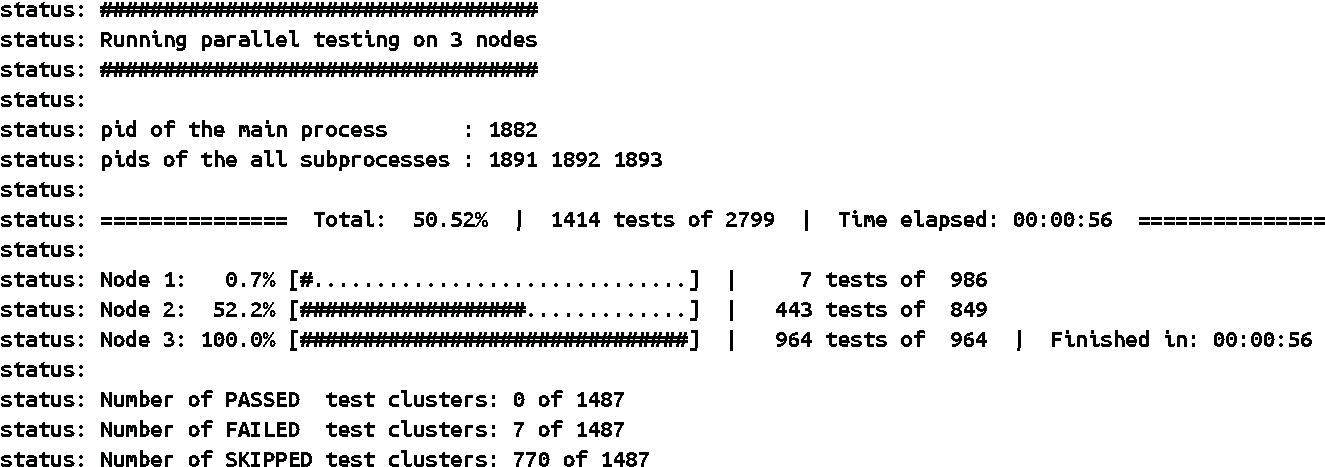
\includegraphics[scale=0.69]{ukazka_progress_baru} 
    \caption{Ukážka progress baru s~väčšou šírkou terminálu}
  \end{center}
\end{figure}



%
% Príloha E
%
\chapter{Prínos práce pre produkt MCO}
\label{priloha:graf_mco}
Nasledujúci graf zobrazuje závislosť medzi počtom použitých testovacích
systémov a~časom potrebným pre otestovanie produktu MCO regresnou 
sadou testov.
Uvedené hodnoty sú vygenerované zo štatistík získaných priamo z~praxe 
pri testovaní produktu MCO.

\begin{figure}[h!]
\begin{tikzpicture}[x=1.4cm,y=0.6cm]

  \def\xmin{1}
  \def\xmax{10}
  \def\ymin{0}
  \def\ymax{16}

  % grid
  \draw[style=help lines, ystep=2, xstep=1] (\xmin,\ymin) grid
  (\xmax,\ymax);

  % axes
  \draw[->] (\xmin,\ymin) -- (\xmax,\ymin) node[right] {počet systémov};
  \draw[->] (\xmin,\ymin) -- (\xmin,\ymax) node[above] {čas [h]};

  % xticks and yticks
  \foreach \x in {1,2,...,10}
    \node at (\x, \ymin) [below] {\x};
  \foreach \y in {2,4,...,16}
    \node at (\xmin,\y) [left] {\y};

  \draw[color=blue] plot[smooth,mark=*,mark size=2pt] file {mco.dat}
   node [right] {MCO};

\end{tikzpicture}
\caption{Závislosť medzi počtom testovacích systémov a~dĺžkou testovania
v~produkte MCO}
\end{figure}



%
% Príloha F
%
\chapter{Prínos práce pre produkt SMSCv5}
\label{priloha:graf_smsc}
Nasledujúci graf zobrazuje závislosť medzi počtom použitých testovacích
systémov a~časom potrebným pre otestovanie produktu SMSCv5 regresnou 
sadou testov.
Uvedené hodnoty sú vygenerované zo štatistík získaných priamo z~praxe 
pri testovaní produktu SMSCv5.

\begin{figure}[h!]
\begin{tikzpicture}[x=1.4cm,y=0.6cm]

  \def\xmin{1}
  \def\xmax{10}
  \def\ymin{0}
  \def\ymax{16}

  % grid
  \draw[style=help lines, ystep=2, xstep=1] (\xmin,\ymin) grid
  (\xmax,\ymax);

  % axes
  \draw[->] (\xmin,\ymin) -- (\xmax,\ymin) node[right] {počet systémov};
  \draw[->] (\xmin,\ymin) -- (\xmin,\ymax) node[above] {čas [h]};

  % xticks and yticks
  \foreach \x in {1,2,...,10}
    \node at (\x, \ymin) [below] {\x};
  \foreach \y in {2,4,...,16}
    \node at (\xmin,\y) [left] {\y};

  \draw[color=blue] plot[smooth,mark=*,mark size=2pt] file {smsc.dat}
   node [right] {SMSCv5};

\end{tikzpicture}
\caption{Závislosť medzi počtom testovacích systémov a~dĺžkou testovania
v~produkte SMSCv5}
\end{figure}
